%%%% IACR Transactions TEMPLATE %%%%
% This file shows how to use the iacrtrans class to write a paper.
% Written by Gaetan Leurent gaetan.leurent@inria.fr (2020)
% Public Domain (CC0)


%%%% 1. DOCUMENTCLASS %%%%
\documentclass[journal=tosc,preprint]{iacrtrans}
%%%% NOTES:
% - Change "journal=tosc" to "journal=tches" if needed
% - Change "submission" to "final" for final version
% - Add "spthm" for LNCS-like theorems

% \usepackage[
% backend=biber,
% style=alphabetic,
% sorting=ynt
% ]{biblatex}

%%%% 2. PACKAGES %%%%
% \usepackage{cite}
\usepackage{algorithmic}
\usepackage{textcomp}
\usepackage{xcolor}
\usepackage{mathtools}

\usepackage{amssymb}
% Language setting
% Replace `english' with e.g. `spanish' to change the document language
\usepackage{times,amsmath,amsthm,amsfonts,eucal,graphicx,listings,booktabs,lipsum,multicol} % Example package -- can be removed

\usepackage[colorlinks=true, allcolors=blue]{hyperref}
\usepackage{enumitem}
\usepackage[T1]{fontenc}
\usepackage{babel}
\usepackage[utf8]{inputenc}
%%%% 3. AUTHOR, INSTITUTE %%%%
\author{Manohar Lal Das \and Aman Khan \and Aayush Deshmukh}
\institute{
  IIT Bhilai, Raipur, India, \email{manoharlal@iitbhilai.ac.in}
  \and
  IIT Bhilai, Raipur, India, \email{amankhan@iitbhilai.ac.in}
  \and
  IIT Bhilai, Raipur, India, \email{aayushd@iitbhilai.ac.in}
}
%%%% NOTES:
% - We need a city name for indexation purpose, even if it is redundant
%   (eg: University of Atlantis, Atlantis, Atlantis)
% - \inst{} can be omitted if there is a single institute,
%   or exactly one institute per author


%%%% 4. TITLE %%%%
\title{PRINT Cipher}
%%%% NOTES:
% - If the title is too long, or includes special macro, please
%   provide a "running title" as optional argument: \title[Short]{Long}
% - You can provide an optional subtitle with \subtitle.

\begin{document}

\maketitle


%%%% 5. KEYWORDS %%%%
\keywords{SPN \and IC-printing}


%%%% 6. ABSTRACT %%%%
\begin{abstract}
  Print Cipher is one of the lightweight SPN network with 48-bit and 96-bit block cipher for IC-printing. It is design to make use of the properties of IC-printing technology. Print cipher is still in the beginning phase of their development but allow the production of different circuits at low cost.
\end{abstract}


%%%% 7. PAPER CONTENT %%%%
\section{Introduction}

In order to identify items using smart bar-codes we use RFID tags and sensors, the security of constrained hardware environments such as RFID tags is major concern in cryptography now a days. PRINTcipher is a 48/96-bit block cipher proposed in CHES 2010 this supports the 80/160-bit secret keys. The key and attractive properties of PRINTcipher are that all rounds use the same round key and differ only by a round counter and that the linear layer is partially key-dependent. The best attack results on PRINTcipher are in-variance subspace attacks on the full \(PRINTcipher-48/96\).\\

Most known cryptanalytic results on PRINTcipher are based on weak keys. The best attack results on PRINTcipher are invariance subspace attacks on the full \(PRINTcipher-48/96\). \(PRINTcipher-48\) attack applicable to \(2^{52}\) weak keys and it requires 5 chosen plaintext with a negligible computational complexity. For \(PRINTcipher-96\) the attack is applicable to \(2^{102}\) weak keys and requires 5 chosen plaintext with a negligible computational complexity.

\begin{figure}[h]
	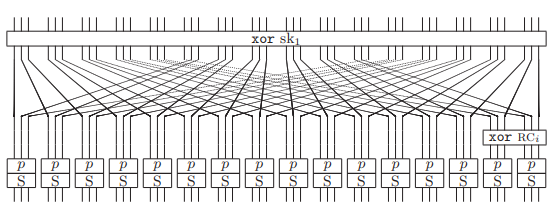
\includegraphics[width=\linewidth]{pics/printcipher.png}
\end{figure}


\section{Main Result}
\label{sec:main}

\subsection{Sbox Analysis}

The sbox for the PRINT cipher is a 3-bit to 3-bit. Since input is 3-bit so for a b-bit block, the sbox is applied $\frac{b}{3}$ parallely. The current state for the sbox is a $\frac{b}{3}$ words, for each word same sbox is used and the next state is the concatenation of outputs.It is a balanced sbox and has a linear structure.The sbox is given in the following table :- \newline

\begin{table}[ht]
	\centering
	\resizebox{10cm}{!}{%
		\begin{tabular}{|l||l|l|l|l|l|l|l|l|}
			\hline
			\multicolumn{1}{|c||}{x} & \multicolumn{1}{c|}{0} & \multicolumn{1}{c|}{1} & \multicolumn{1}{c|}{2} & \multicolumn{1}{c|}{3} & \multicolumn{1}{c|}{4} & \multicolumn{1}{c|}{5} & \multicolumn{1}{c|}{6} & \multicolumn{1}{c|}{7} \\ \hline
			s{[}x{]}                & 0                      & 1                      & 3                      & 6                      & 7                      & 4                      & 5                      & 2                      \\ \hline
		\end{tabular}%
	}
\end{table}

\subsubsection{Difference Distribution Table}
The sbox has a differential branch number defined as min\textsubscript{v, w $\neq$v} \{wt(v $\oplus$ w) + wt(S(v) $\oplus$ S(w))\} of \textbf{2}. The difference distribution table (ddt) which is generated using Sage is as follows :- 
\begin{table}[h]
	\centering
	\resizebox{8cm}{!}{%
		\begin{tabular}{@{}|l|llllllll|@{}}
			\toprule
			& \multicolumn{1}{c}{0} & \multicolumn{1}{c}{1} & \multicolumn{1}{c}{2} & \multicolumn{1}{c}{3} & \multicolumn{1}{c}{4} & \multicolumn{1}{c}{5} & \multicolumn{1}{c}{6} & \multicolumn{1}{c|}{7} \\ \midrule
			0 & 0                     & 0                     & 0                     & 0                     & 0                     & 0                     & 0                     & 0                      \\
			1 & 0                     & 2                     & 0                     & 2                     & 0                     & 2                     & 0                     & 2                      \\
			2 & 0                     & 0                     & 2                     & 2                     & 0                     & 0                     & 2                     & 2                      \\
			3 & 0                     & 2                     & 2                     & 0                     & 0                     & 2                     & 2                     & 0                      \\
			4 & 0                     & 0                     & 0                     & 0                     & 2                     & 2                     & 2                     & 2                      \\
			5 & 0                     & 2                     & 0                     & 2                     & 2                     & 0                     & 2                     & 0                      \\
			6 & 0                     & 0                     & 2                     & 2                     & 2                     & 2                     & 0                     & 0                      \\
			7 & 0                     & 2                     & 2                     & 0                     & 2                     & 0                     & 0                     & 2                      \\ \bottomrule
		\end{tabular}%
	}
\end{table}

\subsubsection{Linear Approximation Table}
The linear branch number which is defined as min\textsubscript{$\alpha$ $\neq$, $\beta$, LAM($\alpha$,$\beta$)$\neq$0}\{wt($\alpha$) + wt($\beta$)\} for this sbox is \textbf{2}. The linearity of this sbox is \textbf{4}. The linear approximation table generated from Sage is as follows:-
% Please add the following required packages to your document preamble:
% \usepackage{graphicx}
\begin{table}[h]
	\centering
	\resizebox{8cm}{!}{%
		\begin{tabular}{|c|cccccccc|}
			\hline
			& 0 & 1  & 2  & 3  & 4  & 5  & 6  & 7  \\ \hline
			0 & 4 & 0  & 0  & 0  & 0  & 0  & 0  & 0  \\
			1 & 0 & -2 & 0  & 2  & 0  & 2  & 0  & 2  \\
			2 & 0 & 0  & 2  & 2  & 0  & 0  & 2  & -2 \\
			3 & 0 & 2  & -2 & 0  & 0  & 2  & 2  & 0  \\
			4 & 0 & 0  & 0  & 0  & 2  & -2 & 2  & 2  \\
			5 & 0 & 2  & 0  & 2  & 2  & 0  & -2 & 0  \\
			6 & 0 & 0  & 2  & -2 & 2  & 2  & 0  & 0  \\
			7 & 0 & 2  & 2  & 0  & -2 & 0  & 0  & 2  \\ \hline
		\end{tabular}%
	}
\end{table}

\subsubsection{Additional Properties of Sbox}
\textbf{1.} The component funcion in 3 variables in algebraic normal form of the sbox is
\begin{center}
	\textbf{x0*x2 + x0 + x1*x2}
\end{center} 

\noindent\textbf{2.} The interpolation polynomial for the sbox is
\begin{center}
	\textbf{(a + 1)x\textsuperscript{6} + (a\textsuperscript{2} + a + 1)x\textsuperscript{5} + (a\textsuperscript{2} + 1)x\textsuperscript{3}}
\end{center}


\noindent\textbf{3. } The polynomials which satisfy the sbox is
\begin{itemize}
	\item x0*x2 + x0 + x1 + y1
	\item x0*x1 + x0 + x1 + x2 + y2
	\item x0*y1 + x0 + x2+ y1 + y2
	\item x0*y2 + x1 + y1
	\item x1*x2 + x0 + y0
	\item x1*y0 + x1 + x2 + y0 + y2
	\item x0*y0 + x1*y1 + x2 + y2
	\item x1*y2 + x0 + x1 + y0
	\item x2*y0 + x1 + y0 + y1
	\item x2*y1 + x0 + y0
	\item x0*y0 + x2*y2 + x0 + x1 + x2 + y0 + y1
	\item y0*y1 + x2 + y0 + y1 + y2
	\item y0*y2 + x1 + y1
	\item y1*y2 + x0+ y0 + y1
\end{itemize}
\hspace{0.5cm} x - input variables y - output variables \newline

\noindent\textbf{4.} Maximum degree of component function - 2\newline

\noindent\textbf{5.} Minimum degree of component function - 2\newline

\noindent\textbf{6.} Maximal differential probability - 0.25\newline

\noindent\textbf{7.} Absolute maximal linear bias - 2\newline

\noindent\textbf{8.} Relative maximal linear bias - 0.25\newline

\subsection{Cryptanalysis of PRINT Cipher}
We are discussing the weakness of PRINTcipher-48/96 on related-key attacks. Related keys that have different values in the part related to a key-dependent permutation. We construct t-round related key differential characteristics with a probability of \(2^{-t}\). By using these characteristics, we can recover the secret keys of \(PRINTcipher-48/96\). To recover the 80-bit secret key of PRINTcipher-48, our attack requires 4 related keys, \(2^{47}\) related-key chosen plaintexts, and a computational complexity of \(2^{60.62}\). In the case of PRINTcipher-96 we require 4 related keys, \(2^{95}\) related-key chosen plaintext and a computational complexity of \(2^{107}\).

\subsection{Construction of Related-Key Differential Characteristics on PRINTcipher}
\subsubsection{Steps to construct  \(t-round\) related-key differential characteristics on printcipher by using properties of a key-dependent permutation KP and S-box}
Related-Key Properties on Key-Dependent Permutation and S-Box:-
3 -bit input value (y\textsubscript{0}, y\textsubscript{1}, y\textsubscript{2}) of a key-dependent permutation of \({KP_l}\). If a 2-bit round key \({s{k^2_l\textsubscript{0}}},{sk^2_l\textsubscript{1}}\) is equal to (0,0) or (0,1)  \\

corresponding output value is computed as follows:
\begin{center}
	(0,0): \(({y_0},{y_1},{y_2})\) $\rightarrow$ \({KP_l}^{00}\) 			  \(({y_0},{y_1},{y_2})\) \\
	(0,1): \(({y_0},{y_1},{y_2})\) $\rightarrow$ \({KP_l}^{01}\) \(({y_1},{y_0},{y_2})\) \\
\end{center}

In the above relations, if \({y_0}\) is equal to \({y_1}\), each permutation outputs the same value and vice versa. That is, the following equation holds:
\begin{center}

\({y_0}\) = \({y_1}\) $\Leftrightarrow$ \({KP_l}^{00}\)\(({y_0},{y_1},{y_2})\) = \({KP_l}^{01}\)\(({y_0},{y_1},{y_2})\)
\end{center}


\textbf{Properties of KP:-}

Consider: \({y_0}\) = \({y_1}\) $\Leftrightarrow$ \({KP_l}^{00}\)\(({y_0},{y_1},{y_2})\) = \({KP_l}^{01}\)\(({y_0},{y_1},{y_2})\)

Consider: \({y_1}\) = \({y_2}\) $\Leftrightarrow$ \({KP_l}^{00}\)\(({y_0},{y_1},{y_2})\) = \({KP_l}^{10}\)\(({y_0},{y_1},{y_2})\)

Consider: \({y_0}\) = \({y_2}\) $\Leftrightarrow$ \({KP_l}^{00}\)\(({y_0},{y_1},{y_2})\) = \({KP_l}^{11}\)\(({y_0},{y_1},{y_2})\)

Consider: \({y_0}\) = \({y_1}\) = \({y_2}\) $\Leftrightarrow$ \({KP_l}^{01}\)\(({y_0},{y_1},{y_2})\) = \({KP_l}^{10}\)\(({y_0},{y_1},{y_2})\)

Consider: \({y_0}\) = \({y_1}\) = \({y_2}\) $\Leftrightarrow$ \({KP_l}^{01}\)\(({y_0},{y_1},{y_2})\) = \({KP_l}^{11}\)\(({y_0},{y_1},{y_2})\)

Consider: \({y_0}\) = \({y_1}\) = \({y_2}\) $\Leftrightarrow$ \({KP_l}^{10}\)\(({y_0},{y_1},{y_2})\) = \({KP_l}^{11}\)\(({y_0},{y_1},{y_2})\)

\subsubsection{Related-Key Differential Characteristics on PRINTcipher-48}

We will apply few property on proposed attack by considering related key-pair: \newline
\((K = (S{K^1},S{K^2}, {K^*} = (S{K^1\textsuperscript{*}},S{K^2\textsuperscript{*}})\)

\(l = 0,....,15\)

\begin{multicols}{3}
	\centering
\textbf{Case 1 (l)}
\(S{K^1}=S{K^1\textsuperscript{*}}\);\\
\(S{K_l^2}=(0,0), S{K_l^2\textsuperscript{*}}=(0,1)\);\\
\(S{K_i^2}=S{K_i^2\textsuperscript{*}}\)where i != l;\\

\textbf{Case 2 (l)}
\(S{K^1}=S{K^1\textsuperscript{*}}\);\\
\(S{K_l^2}=(0,0), S{K_l^2\textsuperscript{*}}=(1,0)\);\\
\(S{K_i^2}=S{K_i^2\textsuperscript{*}}\)where i != l;\\

\textbf{Case 3 (l)}
\(S{K^1}=S{K^1\textsuperscript{*}}\);\\
\(S{K_l^2}=(0,0), S{K_l^2\textsuperscript{*}}=(1,1)\);\\
\(S{K_i^2}=S{K_i^2\textsuperscript{*}}\)where i != l;\\
\end{multicols}


Let input difference of the target round is zero. If key-pair \(K, {k^*}\) satisfies Case 1 (0), \(K{P_0}\) has a nonzero related-key difference. We can construct 1-round related-key differential characteristic \newline 0 $\rightarrow$ \(Case 1 (0)\) 0 with a probability of \(2^{-1}\)under case 1. Since PRINTcipher-48 uses the same round key for all rounds, we can extend this result to a t-round related-key differential characteristic.

\begin{figure}[ht]
	\centering
	\includegraphics[height=8cm, width=12cm]{pics/oneround.png}
	\caption{1-round related-key differential characteristic under Case 1 (0)}
\end{figure}


%\begin{figure}[h!]
	%\centering
	%\subfloat{ \includegraphics[height=5cm, width=7cm]{oneround.png}}
	%\caption{1-round related-key differential characteristic under Case 1 (0)}
%\end{figure}
\newpage
\subsubsection{Related-Key Cryptanalysis on PRINTcipher-48}
we can construct t-round related-key differential characteristics on PRINTcipher-48 with a probability of \(2^{-t}\). These related-key differential characteristics depend on the concrete key value. These related-key differential characteristics depend on the concrete key value. To solve this, we use 4 related keys (\({K_0}^{(0,0)}\), \({K_0}^{(0,1)}\), \({K_0}^{(1,0)}\), \({K_0}^{(1,1)}\)). In detail, two key pairs (\({K_0}^{(0,0)}\), \({K_0}^{(0,1)}\)) and (\({K_0}^{(1,0)}\), \({K_0}^{(1,1)}\)) are considered.

\subsubsection{Basic Related-Key Attack on PRINTcipher-48}
44-round related-key differential characteristic with probability of \(2^{-44}\) is needed to attack full print cipher-48.
Steps for attack procedure:-
\begin{itemize}
	\item Consider plain text strucutres each of four plaintext
	\item Discard the wrong ciphertext pairs from the difference between ciphertexts. For the right ciphertext pair, the output difference of round 45 should be zero.
	\item Guess the partial secret key
	\item Determine related-key pairs satisfying Case 1 (0)
\end{itemize}

\subsubsection{Complexities of Basic Related-Key Attack on PRINTcipher-48}
For plaintext strucutre step computational complexity is  \(2^48\) PRINTcipher-48 encryptions. Next, we discard wrong pair with ciphertext pairs servied is \(2^10(=8.2^{44}.2^{-37})\). Total computational complexity of the attack is \(2^{63}\).

\subsection{Experiment Results}
To demonstrate the efficiency of proposal they have implemented both PRINTcipher variants in VHDL and used Synopsys DesignVision 2007.12 to synthesize them using the Virtual Silicon (VST) standard cell library UMCL18G212T3, which is based on the UMC L180 0.18$\mu$m 1P6M logic process and has a typical voltage of 1.8 Volt.
\begin{figure}[ht]
	\centering
	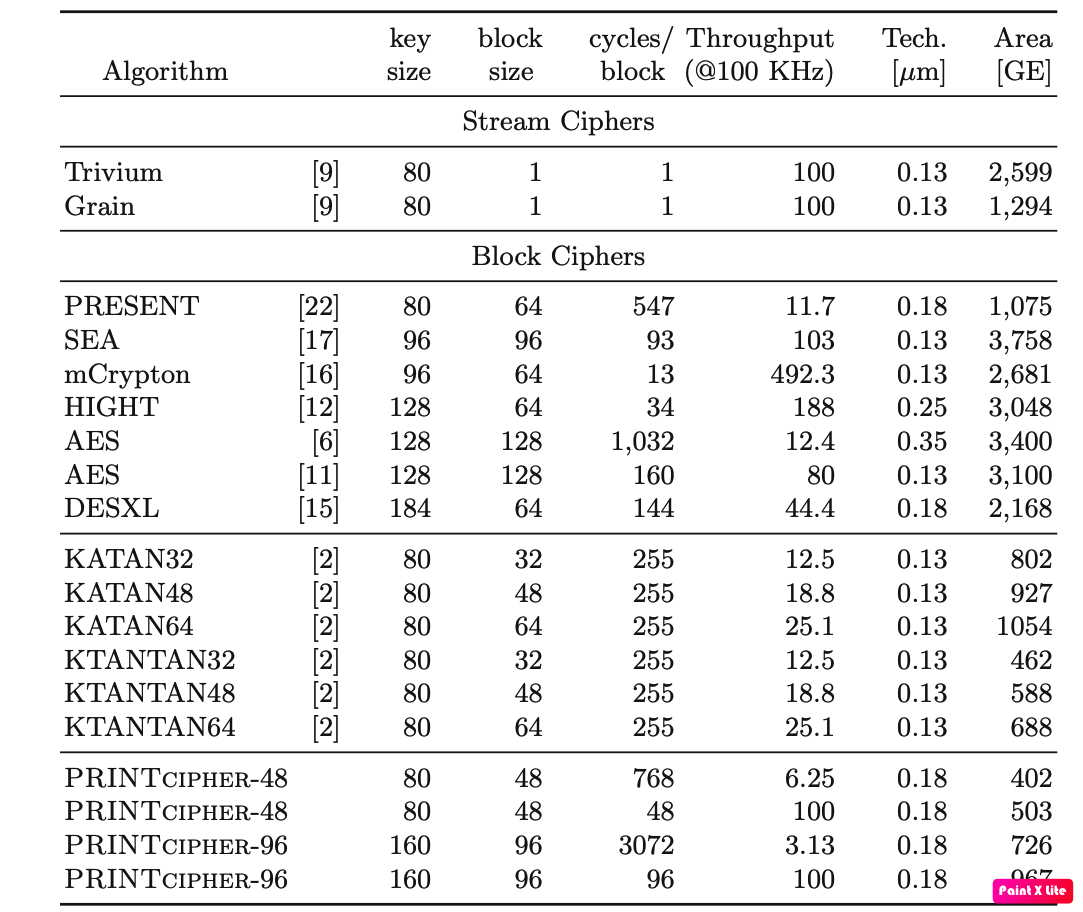
\includegraphics[height=7cm, width=12cm]{pics/hardware.png}
	\caption{Hardware implementation results of some symmetric encryption algorithms.}
\end{figure}

\subsection{Conclusions}
In PRINTcipher they have considered the technology of IC-printing to see how it might influence the  cryptography that we use.They have proposed lightweight block cipher PRINTcipher that explicitly takes advantage of this new manufacturing approach. We related-key cryptanalysis of PRINTcipher.To recover the 80-bit secret key of PRINTcipher-48,related-key differential attack require \(2^47\) related-key chosen plaintexts with a computational complexity of \(2^{60.62}\). Further improvement can be done on the basic related-key attack on the full PRINTcipher-48 by considering 43-round related-key differential characteristics 0 $\rightarrow$ \(Case 1 (0)\) 0.

\subsection{Testvectors}
\begin{figure}[ht]
	\centering
	
\includegraphics[height=1cm, width=5cm]{pics/testvector1.png}
	\caption{Testvector for PRINTcipher-48 in hexadecimal notationAT}
\end{figure}
\newpage
\begin{figure}[ht]
	\centering
	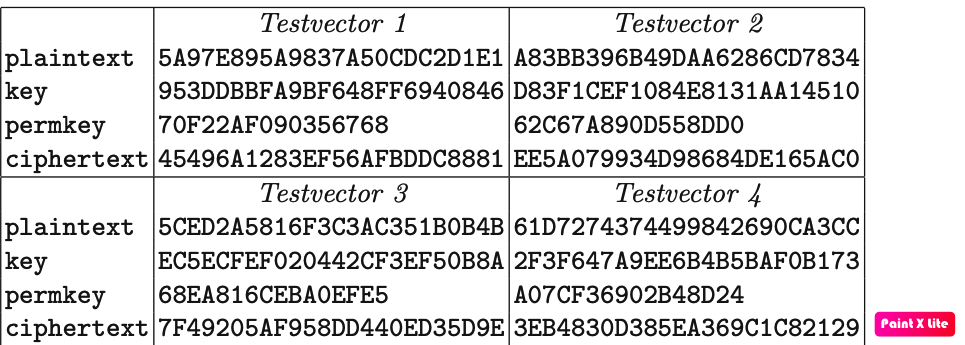
\includegraphics[height=3cm, width=7cm]{pics/testvector-2.png}
	\caption{Testvectors for PRINTcipher-96 in hexadecimal notation}
\end{figure}
\begin{figure}[ht]
	\centering
	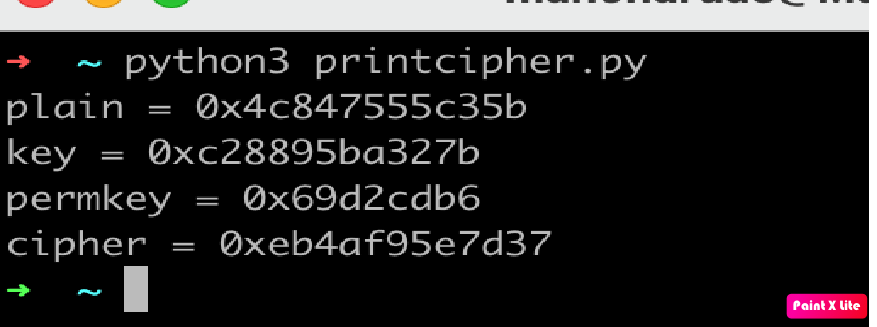
\includegraphics[height=6cm, width=10cm]{pics/pic_1.png}
	\caption{Sage implementation for Encryption of above plaintext}
\end{figure}
\begin{figure}[ht]
	\centering
	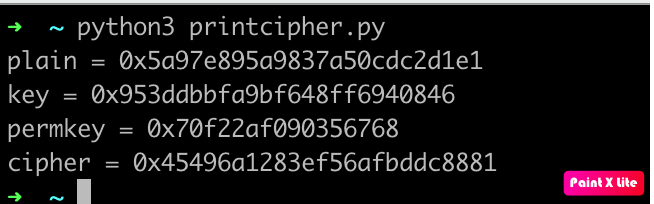
\includegraphics[height=6cm, width=10cm]{pics/pic_2.png}
	\caption{Sage implementation for Encryption of above plaintext}
\end{figure}
\begin{figure}
	\centering
	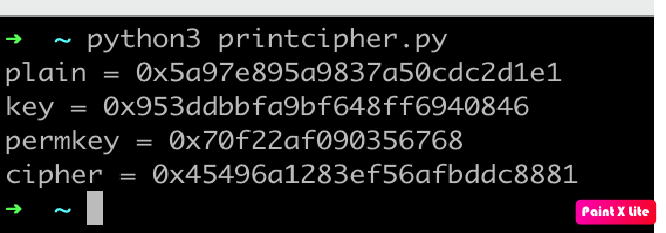
\includegraphics[height=6cm, width=10cm]{pics/pic_3.png}
	\caption{Sage implementation for Encryption of above plaintext}
\end{figure}


\newpage
\subsection{Code Snippet}
\begin{figure}[ht]
	\centering
	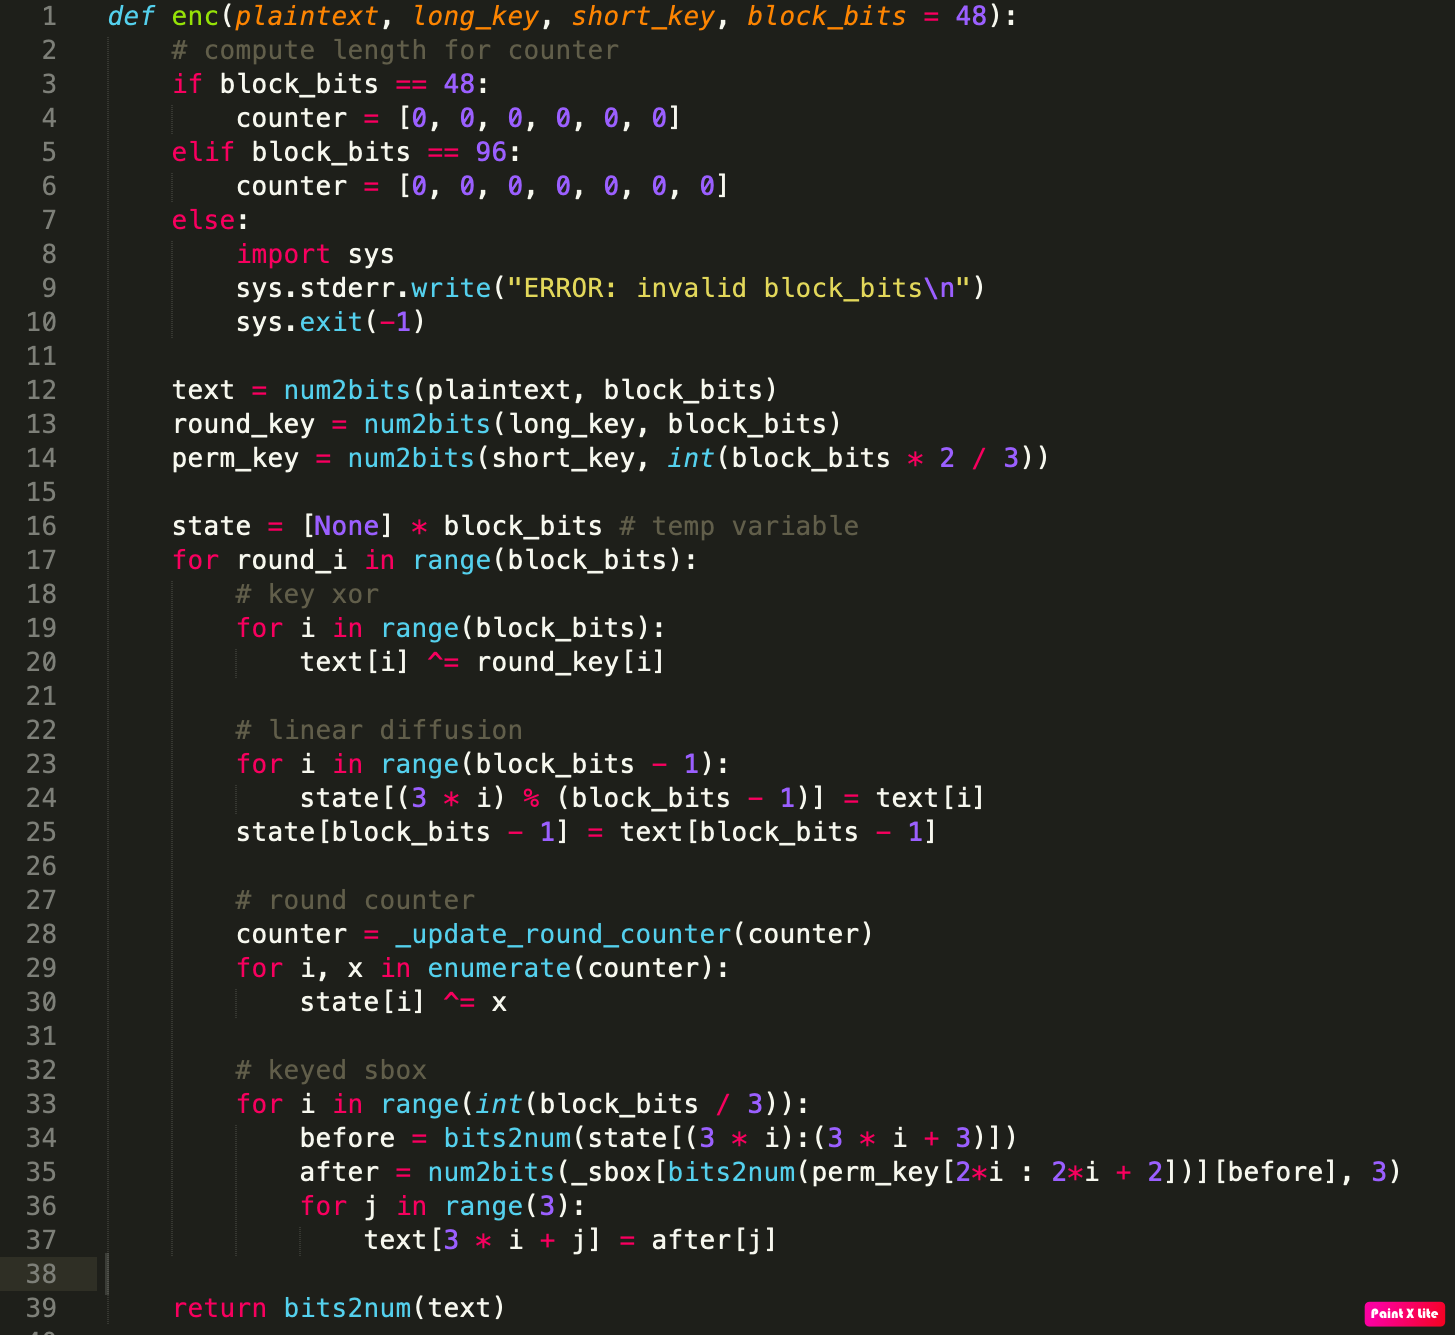
\includegraphics[height=10cm, width=\linewidth]{pics/codesnippet.png}
	\caption{Encryption function of PRINTcipher}
\end{figure}



%%%% 8. BILBIOGRAPHY %%%%
%\bibliographystyle{alpha}
%\bibliography{}
%%%% NOTES
% - Download abbrev3.bib and crypto.bib from https://cryptobib.di.ens.fr/
% - Use bilbio.bib for additional references not in the cryptobib database.
%   If possible, take them from DBLP.

\end{document}
